%% Variational estimator optimization requires a family of distributions to be 
%% optimized over and a method of optimization. In theory, any family can of 
%% distributions can be chosen but often in partice and in this paper, we will 
%% restrict ourselves to the exponential family for many of its convenient 
%% properties. For optimizing within this family, previous work ~\cite{Foster2019}
%% uses a stochastic gradient approach. We suggest a new technique that is unique
%% to the exponential family which provides significant computation time saves by 
%% avoiding expensive gradient steps.

In general, computing the optimal variational estimators
(e.g. $\Imarg$, $\Ipost$, and $\Iml$) requires solving nonlinear--and
often nonconvex--optimization problems.  In the following sections we
demonstrate a class of variational distributions in the exponential
family that correspond to an efficient convex optimization.
Specifically, for Gaussian variational distributions the optimal
estimators can be solved in closed-form by matching expected
sufficient statistics (means and variances).  The same
(efficient) moment calculation yields optimal (or optimal bounded)
estimators for all three cases.  Unless provided, all proofs can be found in the Appendix.

\subsection{Exponential Families}
Our results rely heavily on properties of the exponential family,
which we briefly review here.  A joint distribution $q(x,y)$ is a
member of the exponential family if the PDF / PMF is of the following
form,
\begin{equation}\label{eq:expfam}
  q(x,y) = h(x,y) \exp \left[\eta^TT(x,y)-A(\eta)\right].
\end{equation}
where $\eta$ are the \emph{natural parameters}, $h(x,y)$ is the \emph{base measure},
$T(x,y)$ the \emph{sufficient statistics}, and $A(\eta)$ is the
\emph{log-partition function}.
The exponential family includes many well-known distributions:
Bernoulli, Categorical, Poisson, Gamma, Gaussian, etc.  In addition to
the natural parameters $\eta$ each exponential family has an alternate
set of \emph{mean parameters} $\mu$, defined as the expected
sufficient statistics: $\mu = \mathbb{E}_q[ T(x,y) ]$. Mean parameters
play a key role in finding projections onto the exponential family, as
shown in Lemma~\ref{lemma:MMKL}.
\begin{lemma}[Moment Matching Projection]\label{lemma:MMKL}
  For any distribution $p(x,y)$ and exponential family $q(x,y)$ whose
  support includes that of $p$ the minimum Kullback-Leibler projection:
  \[
    q^* = \argmin_q \, \KL{p(X,Y)}{q(X,Y)}
  = \argmin_q \, \mathbb{E}_p\left[ \log \frac{p(X,Y)}{q(X,Y)} \right]
  \]
  is convex and the solution given by \emph{moment matching} conditions:
  $\mathbb{E}_p[T(X,Y)] = \mathbb{E}_q[ T(X,Y) ] = \mu^*$
\end{lemma}

%% Then \emph{moment matching} is
%% \begin{equation}\label{eq:mm}
%% \E_{p(x,y)}[T(x,y)]=\E_{q(x,y)}[T(x,y)]
%% \end{equation}
%% If we restrict ourselves to the exponential family, then moment matching minimizes 
%% KL divergence. 

The interested reader can consult the texts~\cite{bishop2006pattern,
murphy2012machine} for a proof of Lemma~\ref{lemma:MMKL} and more
details on the exponential family.  In this paper, we will focus on
Gaussian $q(x,y)$. \FIG\ref{fig:GMMex} shows an example of a GMM,
$p(x,y)$, with a moment matched variational Gaussian, $q(x,y)$ (left),
corresponding marginal projection (center), and resulting variational
estimators (right).
\begin{figure*}[!t]
  \centering \subfigure[Joint pdf
  contour]{ 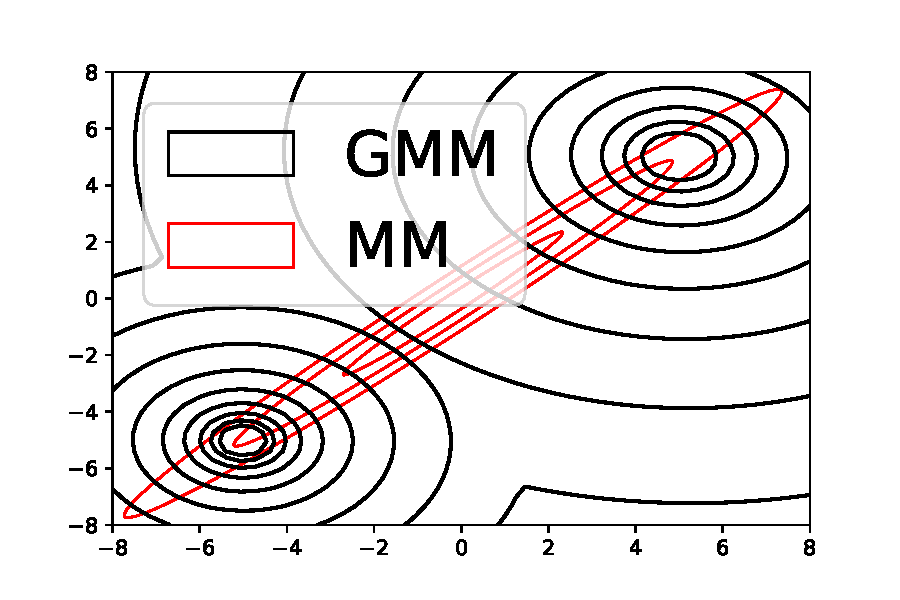
\includegraphics[width=.33\textwidth]{GMMContour.pdf}
  } \subfigure[Marginal
  pdf]{ 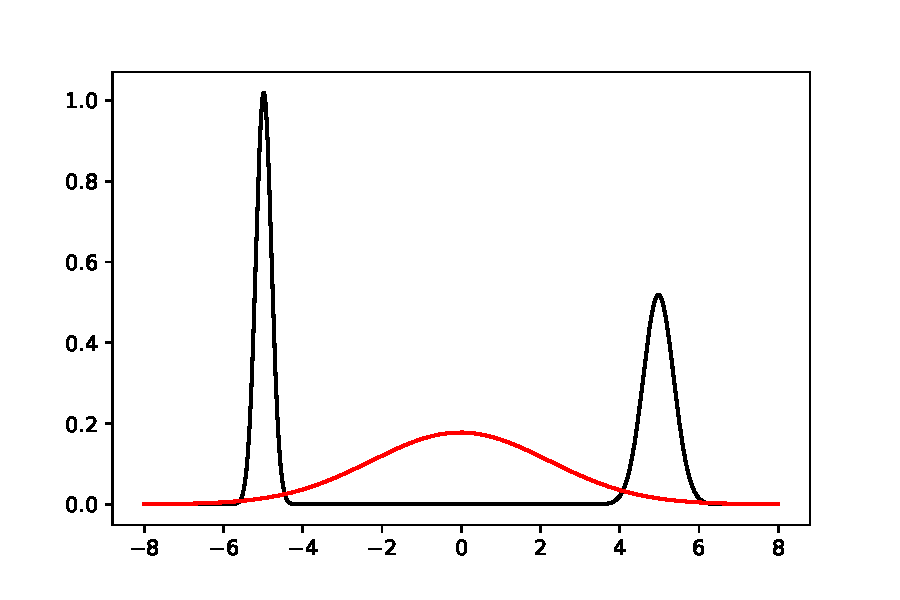
\includegraphics[width=.33\textwidth]{GMMpdf.pdf}
  } \subfigure[MI
  approximations]{ 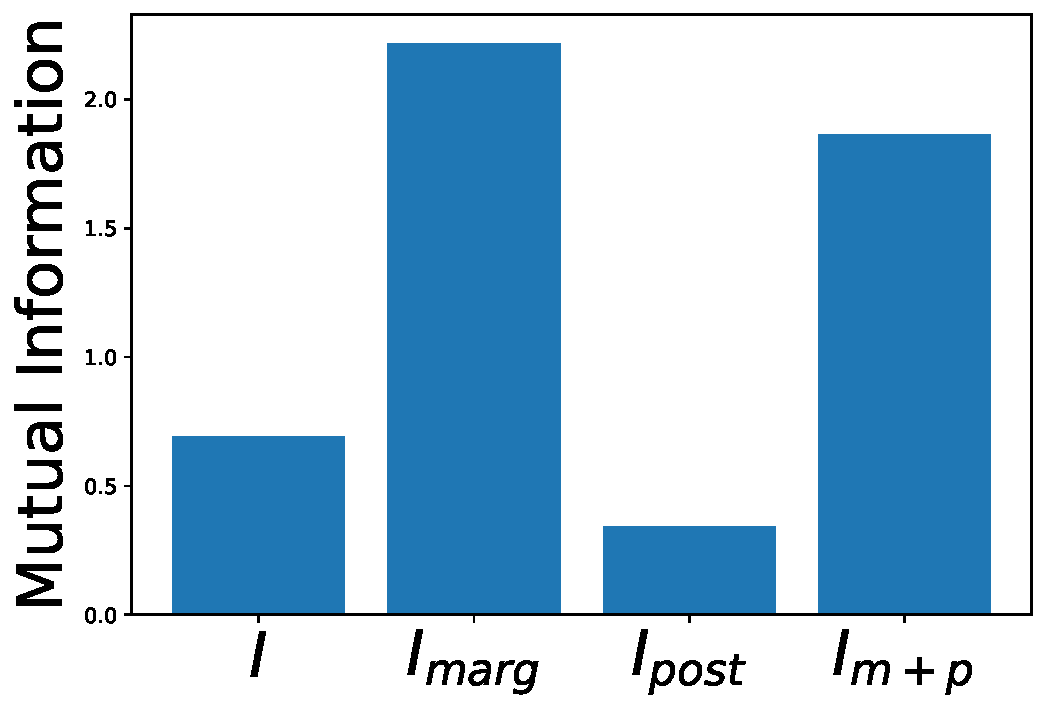
\includegraphics[width=.29\textwidth]{GMMbar.pdf}
  }

  \caption{\small\textbf{Moment Matched Gaussian Mixture Model} (a) A
  bimodal GMM $p$ overlaid with the moment matched Gaussian $q$ has
  its $.5$, $1$, and $1.5$ standard deviation level curves plotted on top in red. (b)
  The marginal PDF is plotted for the Gaussian mixture model and the
  moment matched Gaussian. (c) The true $I(X,Y)$ is shown with
  estimates $\Imarg$, $\Ipost$, and $\Iml$ are all plotted. Notice
  that $\Imarg \geq \Iml \geq \Ipost$.}

  \label{fig:GMMex}
\end{figure*}

%% includes There are many common distributions that fall into this family such as 
%% the Bernoulli distribution, Chi-squared distribution, Wishart distribution, 
%% Gaussian distribution, and many others. Let $q(x,y)$ be in the exponential 
%% family. 

%% The method we propose in this paper matching the moments of a variational 
%% distribution, $q(x,y)$, to those of $p(x,y)$. Our results rely on the properties
%% of the \emph{exponential family}.
%% \begin{definition}{Exponential Family}\\
%%   \emph{
%%   A distribution is a member of the exponential family if it's probability 
%%   density function can be expressed in the form
%%   \[f(x,y|\theta) = h(x,y) \exp \left[\eta(\theta)^TT(x,y)-A(\theta)\right]\]
%%   where $\theta$ are the parameters, $\eta(\theta)$ is the 
%%   natural parameters, $h(x,y)$ is the base measure, $T(x,y)$ is the sufficient 
%%   statistics, and $A(\theta)$ is the log-partition.}
%%   \end{definition}



\subsection{Variational Marginal (upper bound)}\label{sec:varmarg_opt}
To optimize the variational marginal upper bound, $\Imarg$, we must minimze the
bound gap.
\begin{equation}
  I(X;Y) \leq \min_{q_m} \, H_p(q_m(X))-H_p(X \mid Y) = \min_{q_m(X)}H_p(q_m(X)) - \text{const.}
\end{equation}
where the model entropy $H_p(X \mid Y)$ is constant w.r.t. $q_m(x)$
and can be ignored.  If $q_m(x)$ is a Gaussian, then the minimization
is found by moment matching:
\begin{lemma}
  \label{lemma:VMMM} Let $q_m(x)$ be in the exponential family with
  statistics $T(x)$, then for any $p(x,y)$, the optimal $\Imarg^*$ is
  given by moment matching: 
  \[
    \E_{q_m(x)}\left[T(X)\right]=\E_{p(x)}\left[T(X)\right]
  \]  
\end{lemma}
\vspace*{-5mm}\begin{proof} Since $H_p(X)$ is constant in $q_m$ we have,
  \[
    \argmin_{q_m} \, H_p(q_m(X)) = \argmin_{q_m} \,
    H_p(q_m(X))-H_p(X) = \argmin_{q_m} \, \KL{p(X)}{q(Y)}
  \]  
  By Lemma~\ref{lemma:MMKL}, $\E_{q_m(x)}\left[T(X)\right]=\E_{p(x)}\left[T(X)\right]$
  minimizes $\KL{p(X)}{q(Y)}$.
  %% We also know 
  %% $\E_{q(x,y)}\left[T(x,y)\right]=\E_{p(x,y)}\left[T(x,y)\right]$
  %% provides $\E_{q(x)}\left[T(x)\right]=\E_{p(x)}\left[T(x)\right]$.
\end{proof}
Now consider the Gaussian case where $q_m(x)=\Ncal(m,S)$ and a joint
Gaussian $q(x,y)=\Ncal(\mu,\Sigma)$. Moment matching the joint
distribution,
$\E_{q(x,y)}\left[T(X,Y)\right]=\E_{p(x,y)}\left[T(X,Y)\right]$,
provides the marginal moment matching condition. To see this, note
that the marginal moments of the joint are
$q(x)=\Ncal(m_x,\Sigma_{xx})$ where $m_x=m$ is the $x$ component of
the mean and $\Sigma_{xx}=S$ is the block variance of $x$ in $\Sigma$.
Thus, matching the joint Gaussian statistics satisfies
Lemma~\ref{lemma:VMMM} and yields the optimal Gaussian $q_m$ and
corresponding optimal $\Imarg$.



\subsection{Variational Posterior (lower bound)}\label{sec:varpost_opt}
To optimize the variational posterior lower bound, $\Ipost$, we must minimize the
bound gap.
\begin{equation}\label{eq:PostMin}
  I(X;Y) \geq \max_{q_p} \, H_p(X) - H_p(q_p(X \mid Y)) = \min_{q_p} \, H_p(q_p(X \mid Y)) + \text{const}
\end{equation}
The $H_p(X)$ term is constant in $q_p$ and can be ignored for
optimization. The maximization on the left is turned into a
minimization on the right by the negative leading the conditional
entropy.  \EQN\eqref{eq:PostMin} is optimized by satisfying the following
condition,
\begin{lemma}\label{lemma:post_opt}
  If $q_p(x\mid y)$ takes the form of \EQN\ref{eq:ExpFamCond}, then the minimization
  of \EQN\eqref{eq:PostMin} is when
  \begin{equation}\label{eq:OptCrit}
    \E_{p(y)}\left[\E_{q_p(x\mid y)}\left[T(X,Y)\right]\right]=\E_{p(x,y)}\left[T(X,Y)\right]
  \end{equation}
\end{lemma}\vspace*{-2mm}
This result was also shown previously by Pacheco and
Fisher~(\citeyear{pacheco2019variational}).  The condition in
Lemma~\ref{lemma:post_opt} is seemingly a moment matching condition.
However, the l.h.s.~of \EQN\ref{eq:OptCrit} is an expectation
w.r.t.~mixed distributions $p(y)q_p(x\mid y)$, and is difficult to satisfy
in general.  To simplify we consider the joint exponential family
distribution $q(x,y;\eta)$ with natural parameters $\eta$ and
conditional given by,
\begin{equation}\label{eq:ExpFamCond}
  q_p(x\mid y)=q(x\mid y;\eta)=\dfrac{q(x,y;\eta)}{q(y;\eta)}
\end{equation}\label{lemma:OptCrit}
Note that $q(y;\eta)=\int q(x,y;\eta) \, dx$ is not necessarily in the
exponential family.  We can now show that moment matching joint
statistics of $q(x,y;\eta)$ yields the optimal $\Ipost$ via the
following Lemma.
\begin{lemma}\label{lemma:MMOptCrit}
  Let $q_p(x\mid y)$ takes the form of \EQN\ref{eq:ExpFamCond}. Further,
  let the posterior expected statistics be a linear combination of
  marginal statistics as in,\vspace*{-3mm}
  \begin{equation}\label{eq:linearY}
    \E_{q_p(x\mid y)}\left[T(X,Y)\right]=\sum_i^k g_i(\eta)T_{i}(Y)
  \end{equation}
  where $T_i(y)$ is the $i^{th}$ component of the joint statistics
  only depending on  $y$ and $g_i(\eta)$ are arbitrary functions. 
  Then, the optimal $\Ipost$ is given by joint moment matching:
  $\E_{p(x,y)}[ T(X,Y) ] = \E_{q(x,y)}[ T(X,Y) ]$. 
\end{lemma}
Thus both of these conditions imply that moment matching the joint is
optimal for \EQN\eqref{eq:PostMin}. Each of these lemmas are written
in term of an exponential family distribution with some conditions,
since the multivariate Gaussian is the focus of this paper we need to
show that it satisfies these conditions
\begin{corollary}\label{cor:LinearGaussian}
  Let $q(x, y) = \Ncal(m, \Sigma)$ be a Gaussian. Then $q_p(x \mid y)$
  is also Gaussian and satisfies conditions of both
  lemma~\ref{lemma:OptCrit} and lemma~\ref{lemma:MMOptCrit}.
  Furthermore, the optimal $\Ipost$ is obtained by joint Gaussian
  moment matching conditions,\vspace*{-2mm}
  \[
    m^* = \E_{p(x,y)}\left[ (X,Y)^T \right], \qquad \Sigma^* = \text{Cov}_{p(x,y)}\left((X,Y)^T\right)
  \]
  \vspace*{-3mm}And moments of $q_p(x \mid y)$ are the corresponding Gaussian conditional moments
  of $m^*$ and $\Sigma^*$.
\end{corollary}


\subsection{Variational Approximation}\label{sec:varapprox_opt}
Since $\Iml$ is neither an upper nor lower bound, we must minimize the
absolute error
\begin{equation}\label{eq:mi_ml_opt}
  \Iml^* = \argmin_{q_m, q_p} \, \left| I(X;Y) - \Iml(q_m, q_p) \right|
\end{equation}
which is non-convex in general.  We instead minimize the upper bound
as in Foster et al.~(\citeyear{Foster2019}),
\begin{lemma}
  \label{thm:fosterbound} For any model $p(x,y)$ and distributions
  $q_m(x)$, $q_p(x\mid y)$, the following bound holds:
  {\fontsize{9}{10}\selectfont \[\left|\Iml(X,Y)-I(X,Y)\right|\leq
  -\E_{p(x,y)}\left[\log q_m(X)+\log q_p(X\mid Y)\right]+C\]} where
  $C=-H_p(p(X))-H_p(p(X\mid Y))$ does not depend on $q_m$ or
  $q_p$. Further, the RHS is $0$ iff $q_m(x)=p(x)$ and $q_p(x\mid
  y)=p(x\mid y)$ almost surely.  \label{FosterBound2}
\end{lemma}
Previous optimization approaches~\cite{Foster2019} minimize this upper bound using (stochastic) gradient descent:
\begin{equation}\label{eq:sgd_opt}
  q_m^* = \argmax_{q_m} \E_{p(x,y)}[\log(q_m(X))]\hspace{2em}  q_p^* = \argmax_{q_p} \E_{p(x,y)}[\log(q_p(X\mid Y))]
\end{equation}
Note that \EQN\eqref{eq:sgd_opt} does not assume that $q_m(x)$ and
$q_p(x\mid y)$ share a joint distribution $q(x,y)$. We show that under
Gaussianity conditions, not only are optimal $q_m$ and $q_p$ the
marginal and posterior of a joint Gaussian, but that the optimal joint
is found via moment matching.
\begin{theorem}{Equivalence of Moment Matching and Stochastic Gradient Descent}\\
  Let $q_m(x)$ and $q_p(x\mid y)$ be exponential family.  Further, let
  $q_p(x\mid y)$ satisfy the form of \EQN\eqref{eq:ExpFamCond} and the
  linear conditional expectations property (\EQN\eqref{eq:linearY}).
  Then, moment matching the joint distribution $q(x,y)$ yields optimal
  $q_m$ and $q_p$ that minimize the bound on $\Iml$ in
  Lemma \ref{thm:fosterbound}.  \label{EquivMethods}
\end{theorem}
The proof of Theorem~\ref{EquivMethods} (Appendix) follows immediately
from Lemma~\ref{lemma:VMMM} and Lemma~\ref{lemma:MMOptCrit}.
%% says that
%% moment matching the joint minimizes $-\E_{p(x,y)}\left[\log
%% q_m(x)\right]$.  Lemma ~\ref{lemma:OptCrit} and ~\ref{lemma:MMOptCrit}
%% show that moment matching the joint minimizes $-\E_{p(x,y)}\left[\log
%% q_p(x\mid y)\right]$.
Finally, we show that the general result in Theorem
~\ref{EquivMethods} is satisfied for Gaussian $q_m(x)=\Ncal(m,S)$ and
a linear conditional Gaussian $q_p(x\mid y)=\Ncal(Ay+b,\Sigma_p)$
satisfy. 
\begin{corollary}
  Let $q_m(x)=\Ncal(m,S)$ and $q_p(x\mid y)=\Ncal(Ay+b,\Sigma_p)$. Then theorem 
  ~\ref{EquivMethods}  is satsified and thus moment matching a Joint Gaussian 
  $q(x,y)=\Ncal(\mu, \Sigma)$ will minimize lemma~\ref{thm:fosterbound}.
\end{corollary}


\subsection{Properties of Variational Estimators}
We pause here to reflect on the implication of our results
in \SEC\ref{sec:varmarg_opt} - \ref{sec:varapprox_opt}.  Namely, for
joint Gaussian variational $q(x,y)$ all optimality conditions are
satisfied by joint moment matching.  Thus, the same moment-matched
joint Gaussian is optimal for all three variational estimators.  For
the approximation $\Iml$, joint moment matching is equivalent to
optimizing an upper bound on error, but is not globally optimal in
general.  We conclude this section with additional properties of these
estimators.  For example, it is trivial to show that they obey the
following ordering:
%% The $\Imarg$ and $\Ipost$ are often useful because they are bounds. $\Iml$, on 
%% the other hand, is neither an upper bound or lower bound, however this 
%% approximation can be placed between the variational marginal and variational 
%% posterior bounds.\\
\begin{lemma}
  For any $q_m(x)$ and $q_p(x\mid y)$, $\Ipost\leq\Iml\leq\Imarg$.
  \label{lemma:MIOrder}
\end{lemma}
Thus, $\Iml$ is never the least accurate out of all three methods. If
$\Iml$ is an over approximation, it is a tighter upper bound than
$\Imarg$ and the converse holds if it is an under approximation (it is
a tighter than $\Ipost$). We can also ask when $\Iml$ is closer in
absolute error than either of the bounds
\begin{lemma}\label{lemma:AbsPostError}
  For a variational $q_m(x)$ and $q_p(x\mid y)$, if 
  \begin{enumerate}
    \item If $\KL{p(X\mid Y)}{q(X\mid Y)}\geq \frac{1}{2}\KL{p(X)}{q(X)}$ 
    then $\Iml$ has lower error than $\Ipost$
    \item If $\KL{p(X)}{q(X)}\geq \frac{1}{2}\KL{p(X\mid Y)}{q(X\mid Y)}$ 
    then $\Iml$ has lower error than $\Imarg$
  \end{enumerate}
\end{lemma}
While these conditions cannot be checked in practice they do offer
some insight.  For example, if $q_m(x)$ approximates $p(x)$ about as
well as $q_p(x\mid y)$ approximates $p(x\mid y)$ (in KL) then $\Iml$ is the
best approximation to use.

\paragraph{Moment matching stationary point} is not always a local minimum to the 
optimization of $\Iml$. Consider \FIG\ref{fig:MMoptimal} where a two
dimensional Gaussian is moment matched to Gaussian mixture models. All
of the parameters of the moment matched Gaussian are held constant but
the correlation parameter, $\rho$, is varied an the absolute error of
$\Iml$ is plotted. In one case, the minimum is found and any changed
value of $\rho$ results in a worse approximation of MI. However is the
second case, a local maximum is found, and we notice that there is a
range of values for $\rho$ that result in not only better
approximations of MI, but sometimes exact.  Exploring this property is
a topic of future work.

\begin{figure*}[!t]
  \centering
  \subfigure[Local minimum]{
    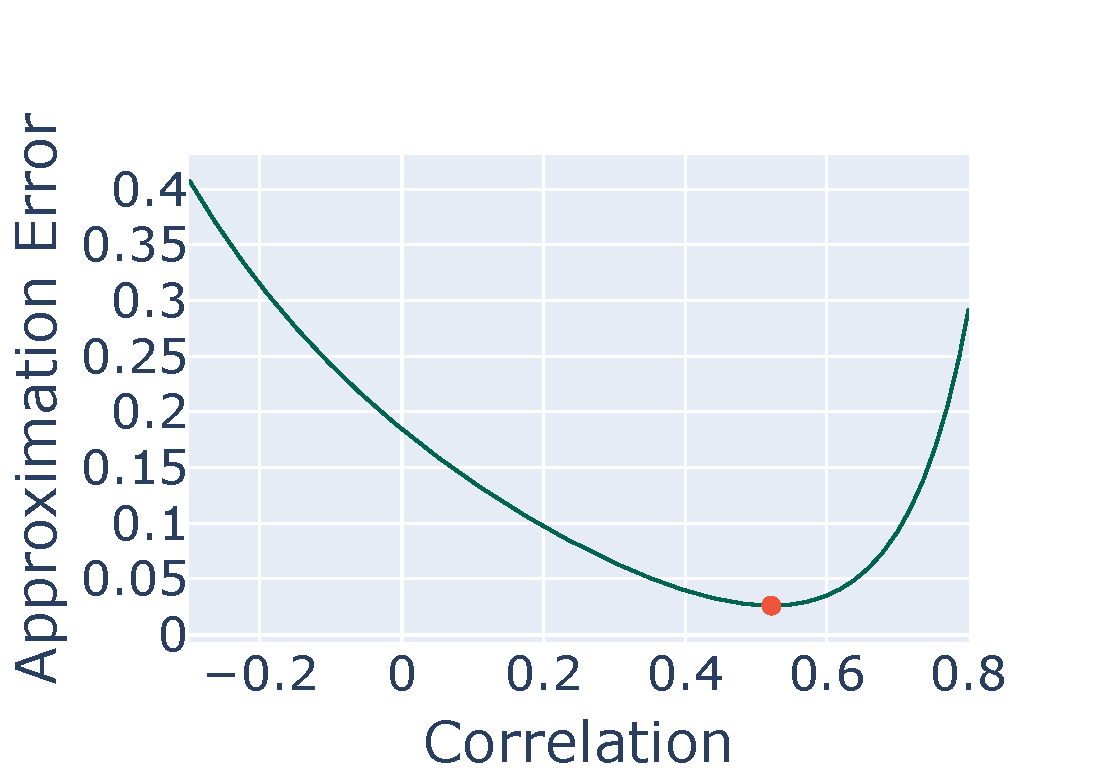
\includegraphics[width=.4\textwidth]{MMMinimum.pdf}
    }
  \subfigure[Local maximum]{
  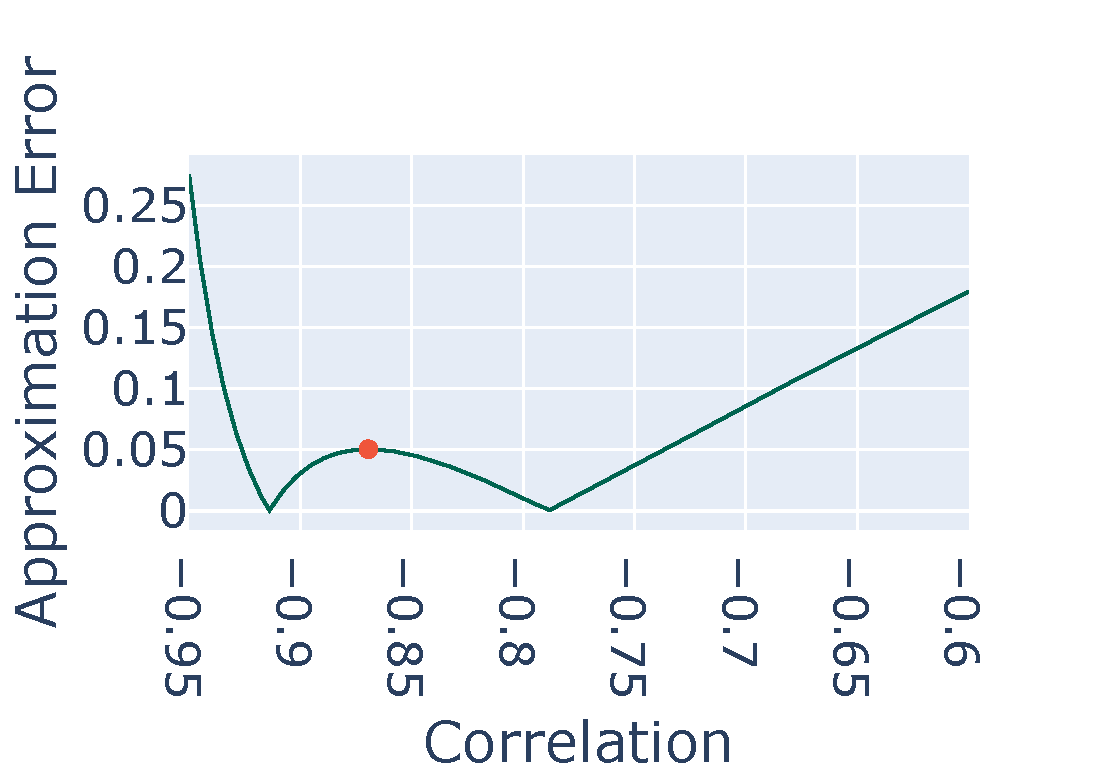
\includegraphics[width=.4\textwidth]{MMMaximum.pdf}
  }
  \caption{\small\textbf{Moment Matched Optimum} (a) The moment matching solution 
  (red) is the local minimum as a variational apprximation to a GMM. (b) For a 
  seperate GMM, the moment matched solution is a local maximum and there is a 
  range of values for $\rho$ that result in better approximation, and two that 
  result in exact values of MI.}
  \label{fig:MMoptimal}
\end{figure*}



% Each variation method has its own error which must be minimized, $\Imarg$ has 
% an error of $KL(p(x)||q(x))$, $\Ipost$ has an error of $KL(p(x|y)||q(x|y))$, 
% and $\Iml$ has an error of $KL(p(x)||q(x))-KL(p(x)||q(x))$. Finding the best 
% approximation $\Iml$ requires minimizing the approximation error,
% \begin{equation}\label{eq:mi_ml_opt}
%   \Iml^* = \argmin_{q_m, q_p} \, \left| I(X;Y) - \Iml(q_m, q_p) \right|
% \end{equation}
% which cannot be computed in general.  Foster et
% al.~(\citeyear{Foster2019}) instead minimize an upper bound provided
% in the following lemma,
% \begin{lemma}
%   \label{thm:fosterbound}  
%   For any model $p(x)p(y|x)$ and distributions $q_m(x)$ and
%   $q_p(x|y)$, the following bound holds:
%   {\fontsize{9}{10}\selectfont
%     \[\left|\widetilde{I}(x,y)-I(x,y)\right|\leq -\E_{p(x,y)}\left[\log q_m(x)+\log q_p(x|y)\right]+C\]}
%   where $C=-H_p(p(x))-H_p(p(x|y))$ does not depend on $q_m$ or
%   $q_p$. Further, the RHS is $0$ iff $q_m(x)=p(x)$ and
%   $q_p(x|y)=p(x|y)$ almost surely.
%   \label{FosterBound2}
% \end{lemma}
% A proof of Lemma~\ref{thm:fosterbound} is reproduced in the appendix. 
% \paragraph{Optimization methods} suggested by previous work ~\cite{Foster2019} is
% \emph{stochastic gradient descent}.
% \begin{equation}\label{eq:sgd_opt}
%   q_m^* = \argmax_{q_m} \E_{p(x,y)}[log(q_m(x))]\hspace{2em}  q_p^* = \argmax_{q_p} \E_{p(x,y)}[log(q_p(x|y))]
% \end{equation}
% Lemma ~\ref{thm:fosterbound} is found by seperately finding $q_m^*$ and $q_p^*$ by 
% equation \ref{eq:sgd_opt}. For $\Imarg$, the optimal distribution is found by 
% just finding $q_m^*$ and the optimal distribution for $\Ipost$ is just $q_p^*$.


% \subsection{Optimizing $\Iml$}
% To minimize the bound in Lemma~\ref{thm:fosterbound}, an optimal 
% marginal, $q_m$ and posterior, $q_p$, must be found.

% \subsubsection{Stochastic Gradient Descent}
% Previous work suggests finding the maximum by separately optimizing a Gaussian 
% marginal $q(x)=q_m(x)$ and Gaussian posterior $q(x|y)=q_p(x|y)$ though stochastic 
% gradient ascent. That is he separately calculates the following:
% \begin{equation}\label{eq:sgd_opt}
%   q_m^* = \argmax_{q_m} \E_{p(x,y)}[log(q_m(x))]\hspace{2em}  q_p^* = \argmax_{q_p} \E_{p(x,y)}[log(q_p(x|y))]
% \end{equation}
% It is important to note that this does not assume that $q_m(x)$ and $q_p(x|y)$ share 
% a joint Gaussian, $q(x,y)$, that they are both derived from. This approach will 
% find our optimal distribution to minimize the bound in Lemma~\ref{thm:fosterbound} 
% however this requires two optimization operations to be computed which can be 
% time consuming, especially with higher dimensional problems.

% \subsubsection{Moment Matching}
% The method proposed in this paper, instead of computing Gradient Descent, we will
% match the moments of $q(x,y)$ to those of $p(x,y)$. To define what this means, 
% we first intrduce the \emph{Exponential Family}
% \begin{definition}{Exponential Family}\\
%   \emph{
%   A distribution is a member of the Exponential Family if it's probability 
%   density function can be expressed in the form
%   \[f(x,y|\theta) = h(x,y) \exp \left[\eta(\theta)^TT(x,y)-A(\theta)\right]\]
%   where $\theta$ are the parameters, $\eta(\theta)$ is the 
%   Natural Parameters, $h(x,y)$ is the base measure, $T(x,y)$ is the sufficient 
%   statistics, and $A(\theta)$ is the Log-partition.}
%   \end{definition}
% There are many common distributions that fall into this family such as 
% the Bernoulli distribution, Chi-squared distribution, Wishart distribution, 
% Gaussian distribution, and many others. The case of the Multivariate Gaussain
% will be the focus of this paper but results can be expanded to include other 
% distributions from the exponential family as well.

% Let $q(x,y)$ be in the Exponential Family. Then \emph{Moment Matching} is
% \begin{equation}
% \E_{p(x,y)}[T(x,y)]=\E_{q(x,y)}[T(x,y)]
% \end{equation}
% and the resulting marginal and likelihood are used as the approximating distributions
% \begin{align}\label{eq:mm_opt}
% q_m^*(x)=q_\eta(x)=\int q_\eta(x,y)dy \hspace{2em} q_p^*(x|y)=q_\eta(x|y)=\dfrac{q_\eta(x,y)}{\int q_\eta(x,y)dx}
% \end{align}
% In this paper, we will focus on the case where $q(x,y)$ is the Multivariate 
% Gaussiian in the exponential family. Figure ~\ref{fig:GMMex} shows an example of 
% a Gaussian Mixture Model, $p(x,y)$, with a moment matched variational Gaussian, 
% $q(x,y)$. Notice that the moment matching finds the mean of the nodes and then 
% matches the varaiance to capture both nodes. This Gaussian is then used as the 
% variational distribution for each of the variational methods and their outputs 
% compared. The ordering of each method matches Lemma ~\ref{lemma:MIOrder}.
% We will show that for Gaussian variational families, the optimal $q_m$ 
% and $q_p$ found in equation \ref{eq:sgd_opt} share a unique optimal joint. 
% We further show that the optimal joint distribution is given by moment matching.
% \begin{figure*}[!htb]
%   \centering
%   \subfigure[Joint pdf contour]{
%   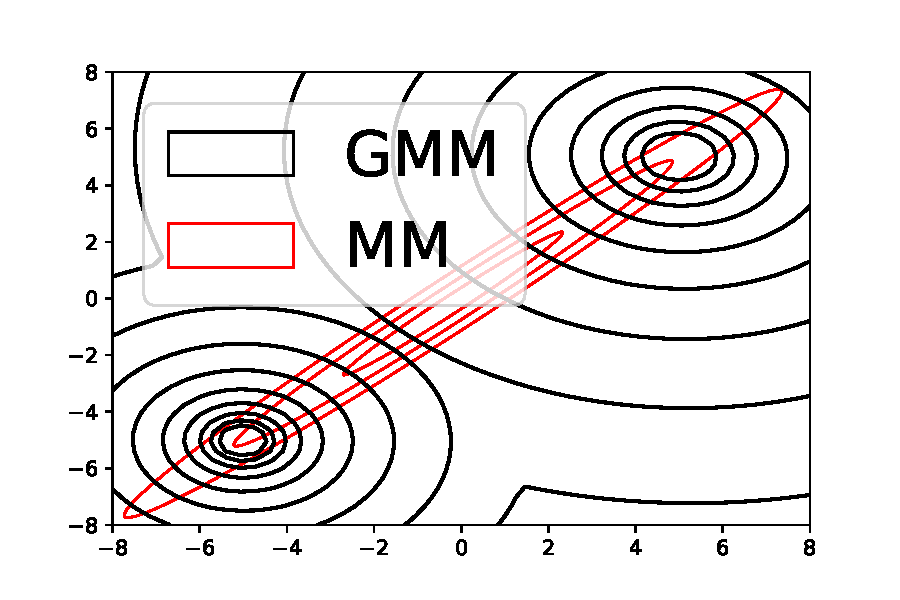
\includegraphics[width=.33\textwidth]{GMMContour.pdf}
%   }
%   \subfigure[Marginal pdf]{
%   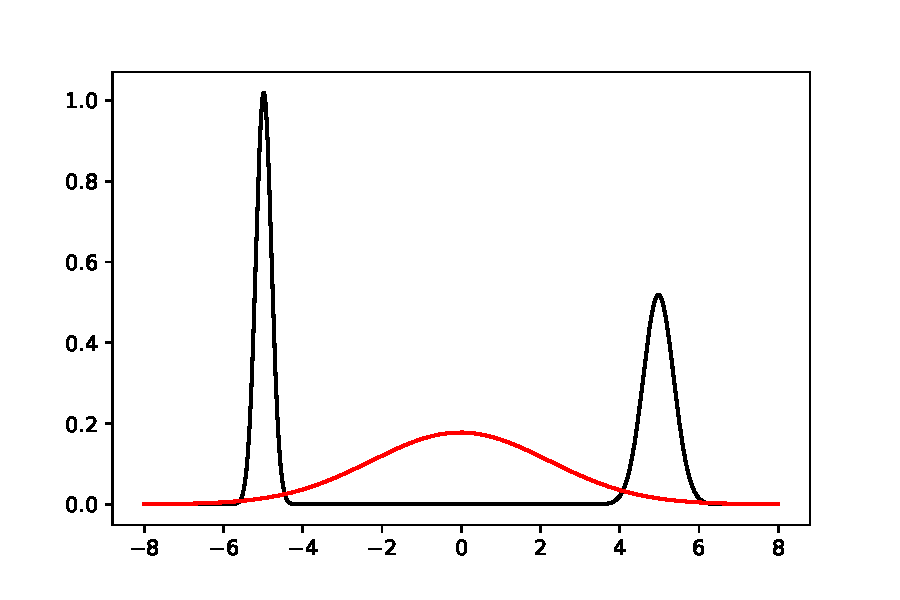
\includegraphics[width=.33\textwidth]{GMMpdf.pdf}
%   }
%   \subfigure[MI approximations]{
%   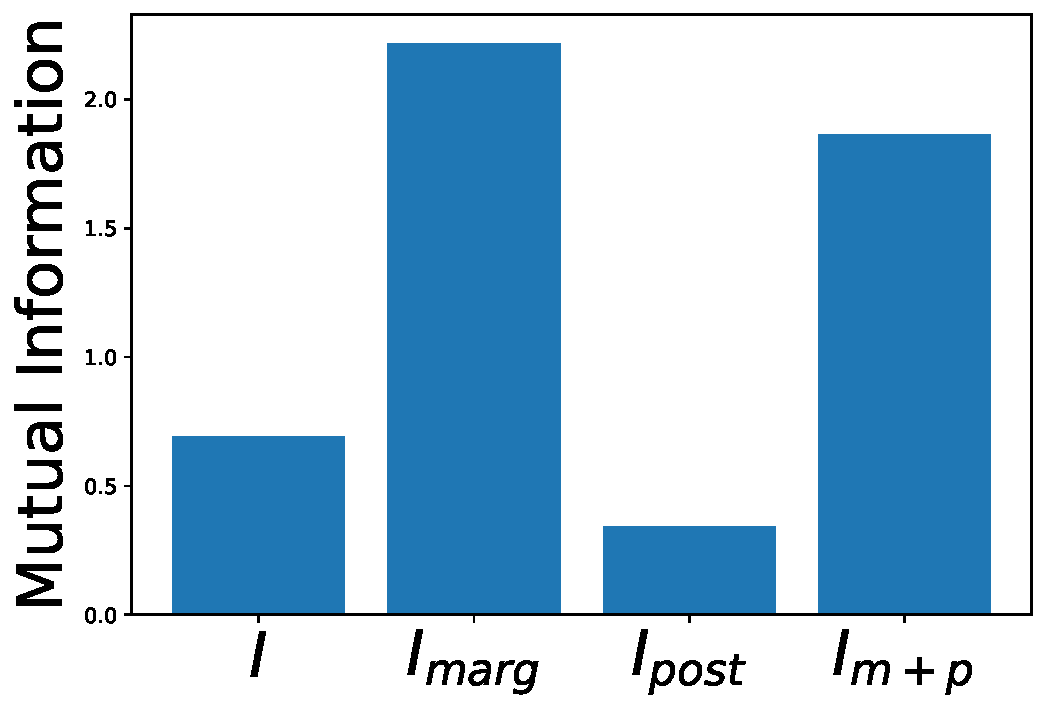
\includegraphics[width=.29\textwidth]{GMMbar.pdf}
%   }
%   \caption{\small\textbf{Moment Matched Gaussian Mixture Model} (a) A Gaussian Mixture 
%   Model with two means is plotted and its level curves. The moment matched 
%   Gaussian has its one standard deviation level curve plotted on top in red. (b)
%   The marginal pdf of the Latent Variable is plotted for the Gaussian Mixture 
%   Model and the moment matched Gaussian. The Gaussian is mean-seeking instead 
%   of mode seeking (c) The True $I(X,Y)$, $\Imarg(X,Y)$, $\Ipost(X,Y)$, and 
%   $\Iml(X,Y)$ are all plotted. Notice that $\Imarg(X,Y)\geq\Iml(X,Y)\geq\Ipost(X,Y)$ 
%   as expected.}
%   \label{fig:GMMex}
%   \end{figure*}

% \subsubsection{Equivalence of Methods}
% We first show that there exists a shared joint, $q(x,y)$, that generates 
% both $q_m$ and $q_p$. If this holds, then the stochastic gradient decent 
% approach can be reduced from minimzing two distribution to just one.\\

% \begin{lemma}{Uniqueness of Multivariate Gaussian}\\
%   For any linear conditional Gaussian variation distribution of the form 
%   $q(X|y)=N(Ay+b|\Sigma)$ where $\Sigma$ is independent of $y$, then there exists a 
%   unique joint Gaussian, $q(x,y)$, for any Gaussian marginal distribution $q(x)$.
%   \label{UniqueGaussian}
% \end{lemma}
% This tells us the assumption of $q_m$ and $q_p$ not sharing a joint Gaussian 
% is unnecessary as there exists a unique joint Gaussian that will produce any 
% separate $q_m$ and $q_p$. This reformulates equation ~\ref{eq:sgd_opt} To
% \begin{equation}
%   q^*(x,y) = \argmax_{q(x,y)}\left(\E_{p(x)}[\log(q(x))]+\E_{p(x,y)}(\log(q(x|y)))\right)
% \end{equation}

% \begin{theorem}{Equivalence of Moment Matching and Gradient Methods for Variational Gaussian}\\
%   Let $q_\eta(x,y)=N(\mu,\Sigma)$, $q_\eta(x)=\int q_\eta(x,y)dy$, 
%   and $q_\eta(x|y)=\dfrac{q_\eta(x,y)}{q_\eta(y)}$, where $\eta$ are the exponential 
%   family parameters of the joint Gaussian and $T(x,y)$ are the sufficient statistics. Then
% \[\E_{p(x,y)}[T(x,y)]=\E_{q(x,y)}[T(x,y)]\]
%   finds the same minimum as gradient ascent of
%   \[-\E_{p(x,y)}\left[log(q_\eta(x))+log(q_\eta(x|y))\right]\]
%   \label{EquivMethodsGauss}
% \end{theorem}

% The proof of Theorem \ref{EquivMethodsGauss} can be found in the appendix.\\ 
% Theorem~\ref{UniqueJoint} and Theorem~\ref{EquivMethodsGauss} together tell us 
% that if we are working with a Multivariate Gaussian variational distribution, 
% then Moment Matching is equivalent to Gradient Descent for minimizing the bound 
% in Theorem~\ref{thm:fosterbound}.\\

% \subsection{Properties of Variational Estimators}
% The $\Imarg$ and $\Ipost$ have nice properties that we can bound them relative 
% to the True MI. $\Iml$, on the other hand, is neither an upper bound or lower 
% bound due to bounding both entropy terms. However this approximation can be placed
% between the Variational Marginal and Variational Posterior bounds.\\
% \begin{lemma}
%   For any variational distributions $q_m(x)$ and $q_p(x|y)$, the following holds
%   \[\Ipost\leq\Iml\leq\Imarg\]
%   \label{lemma:MIOrder}
% \end{lemma}
% The proof of this lemma can be found in the appendix. However it is simple to see 
% that this must be true. The error of equation \ref{eq:mi_marg} is $KL(p(x)||q(x))$
% and the error of equation \ref{eq:mi_ml} is $KL(p(x)||q(x))-KL(p(x|y)||q(x|y))$ 
% which is error of the variational marginal minus a postive KL Divergence, 
% making it smaller than the upper bound. A similar argument holds to show that
% $\Iml$ is larger than the lower bound. \\
% Lemma ~\ref{lemma:MIOrder} always holds regardless of the model, however we can 
% ask when $\Iml$ is closer in absolute error to the true MI than either of the 
% bounds. Consider $\Ipost$, which has error $KL(p(x|y)||q(x|y))$
% \begin{equation}\label{eq:AbsPostError}
%   \left|KL(p(x|y)||q(x|y))\right|\geq \left|KL(p(x)|q(x))-KL(p(x|y)||q(x|y))\right| \Rightarrow 2KL(p(x|y)||q(x|y))\geq KL(p(x)||q(x))
% \end{equation}
% Equation ~\ref{eq:AbsPostError} shows us that $\Iml$ is closer in absolute error 
% to the true MI than $\Ipost$ if $2KL(p(x|y)||q(x|y))\geq KL(p(x)|| q(x))$. 
% Following a similar argument, $\Iml$ is close to the true MI than $\Imarg$ If
% $2KL(p(x)||q(x))\geq KL(p(x|y)||q(x|y))$. Neither of these conditions can be 
% checked in practice as True entropy terms need to be calculated to evalute these
% KL divergences, however this can be used to make Hueristic arguments for when $\Iml$ 
% is a good approximation. If $q(x)$ approximates $p(x)$ about as well as $q(x|y)$ 
% approximated $p(x|y)$, then $\Iml$ is better to use in all cases.\\
% \begin{figure*}[!htb]
%   \centering
%   \subfigure[Local minimum]{
%     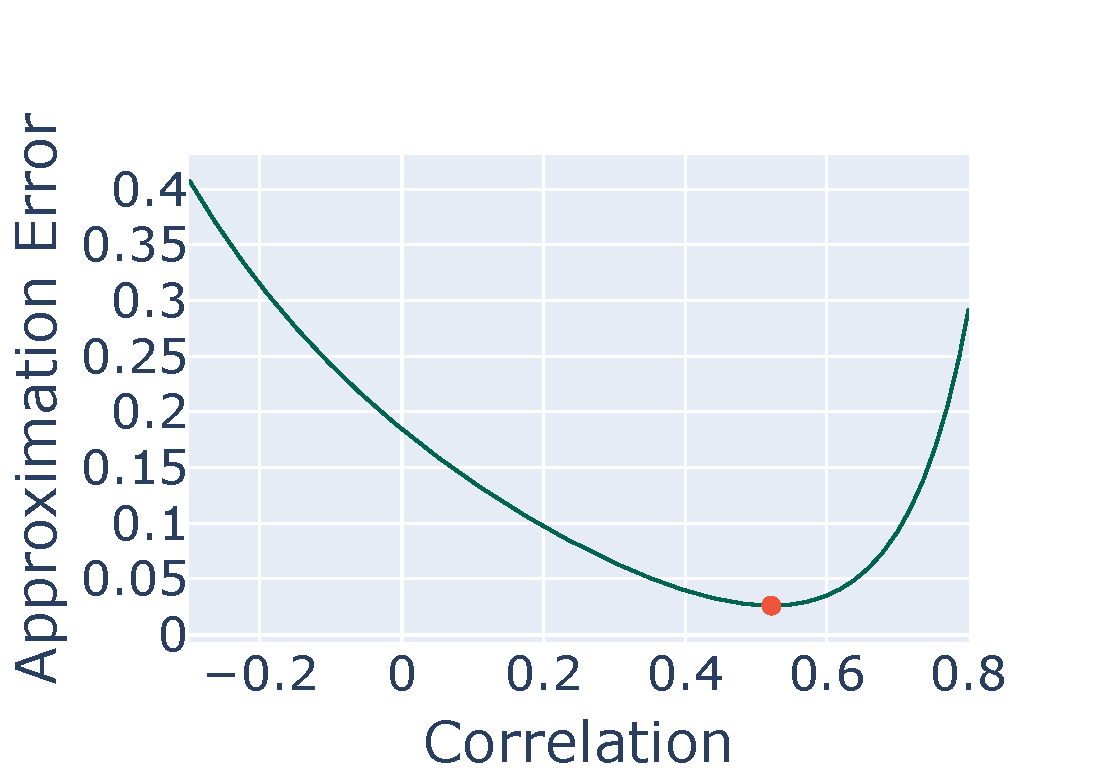
\includegraphics[width=.31\textwidth]{MMMinimum.pdf}
%     }
%   \subfigure[Local maximum]{
%   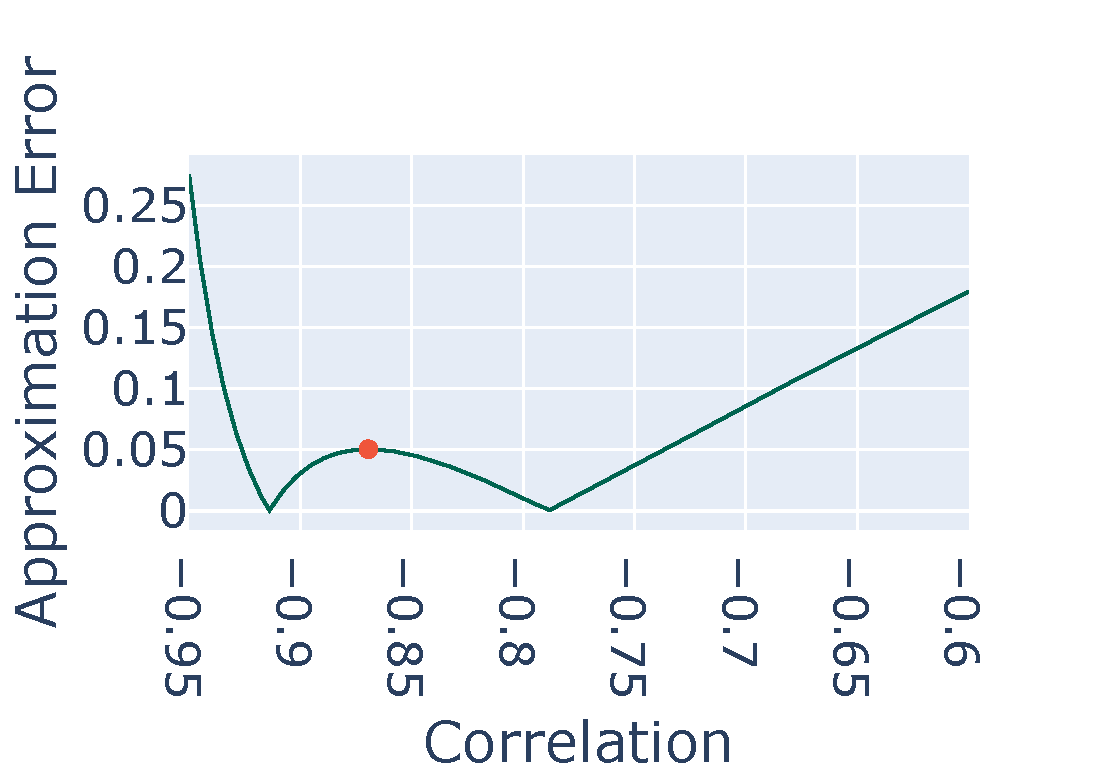
\includegraphics[width=.31\textwidth]{MMMaximum.pdf}
%   }
%   \caption{\small\textbf{Moment Matched Optimum} (a) In this case, a GMM is MM and then
%   the value of $\rho$ is varied. The Moment matching solution (red), is the local
%   minimum and no better values of $\rho$ exist. (b) Another GMM is MM, in this case
%   the moment matched solution finds a local maximum and there is a range of values
%   for $\rho$ that result in better approximation, and two that result in exact 
%   values of MI.}
%   \label{fig:MMoptimal}
%   \end{figure*}
% Another interesting property to note is that Moment Matching does not always find 
% a local minimum to the optimization of the variational distribution. Conisder 
% Figure ~\ref{fig:MMoptimal} where Gaussian Mixture Models are moment matched to a
% Gaussian. All of the paramters of the Moment Matched Gaussian is held constant but
% the correlation parameter, $\rho$, is plotted versus the absolute error to the True
% MI. In one case, the minimum is found and any changed value of $\rho$ results in a
% worse approximation of MI. However is the second case, a local maximum is found, 
% and we notice that there is a range of values for $\rho$ that result in not only
% better approximations of MI, but sometimes exact.\\

% \subsection{Optimizing $\Imarg$ and $\Ipost$}
% We now observe how to optimize Equation \ref{eq:mi_marg} and \ref{eq:mi_post}.
% Previously, the optimal distribution was found by minimizing the error $KL(p||q)$
% via a stochastic gradient methods, however, appealing to distributions in the 
% Exponential Family, this optimiziaiton can be simplified
% \begin{theorem}{Moment Matching Minimizes KL}
%   For any distribution, $p(x,y)$, and a Gaussian variational distribution, $q(x,y)$, 
%   the KL divergence, $KL(p(x)||q(x))$ and $KL(p(x|y)||q(x|y))$, are minimized 
%   by moment matching the joint.
%   \[E_p[T(x,y)]=E_q[T(x,y)]\]
%   \label{th:KLMin}
% \end{theorem}
% Because $\Imarg$ has an error of $KL(p(x)||q(x))$ and $\Ipost$ has an error 
% of $KL(p(x|y)||q(x|y))$, Moment Matching a Gaussian variational distribution 
% will minimze the $KL$ error of both methods and thus optimize the Variational 
% Marginal and Variational Posterior bounds. This means that when we moment match 
% a joint Gaussian, the resulting distribution will optimize $\Imarg$, $\Ipost$, 
% and $\Iml$ at the same time.

% \subsection{Generalize Proofs of Optimization}
% The results of Theorem \ref{UniqueGaussian} and Theorem \ref{EquivMethodsGauss}
% can be extended to include more general distributions as well. Theorem 
% \ref{UniqueGaussian} is extended in Seshadri and Patil \ref{SeshadriPatil}

% \begin{theorem}{Unique Joint Condition}\\
%   Given $f_x(x)$ and $f_{x|y}(x|y)$, a sufficient condition for
%   $f_y(y)$ (and hence for $f_{x,y}(x,y)$) to be unique is that the
%   conditional p.d.f. of $x$ given $y$ is of the exponential form
%   \[f_{x,y}(x|y)=exp\left[yA(x)+B(x)+C(y)\right]\]
%   where an interval is contained in the range of $A(x)$.
%   \label{UniqueJoint}
% \end{theorem}

% This generalizes the conditional distribution form being a linear Gaussian to 
% simply being in the exponential family and having a cross term tha tis linear 
% in $y$.\\
% Theorem \ref{EquivMethodsGauss} can be extend to further include other member of
% the exponential family.
% \begin{theorem}{Equivalence of Moment Matching and Stochastic Gradient Descent}
%   Let $q_m(x)$ and $q_p(x|y)$ share a common joint in the exponential family,

%   \[q_\eta(x,y)=h(x,y) \exp \left[\eta^TT(x,y)-A(\eta)\right]\]

%   Also assume linear conditional expectations of the sufficient statistics

%   \[\E_{q(x|y)}\left[T(x,y)\right]=\sum g_i(\eta)T_i(y)\hspace{2em} \E_{q(y|x)}\left[T(x,y)\right]=\sum h_i(\eta)T_i(x)\]

%   Then Moment Matching finds the same minimum as gradient ascent of Theorem \ref{thm:fosterbound}.
%   \label{EquivMethods}
% \end{theorem}
